The questionnaire survey was created, mainly, to figure out some more precise weights for how people choose the media they want to consume. So not only as a way to validate the results from the interview survey, but also as variables to implement later in a solution.
In total, the questionnaire received 82 responses from 52 males and 30 females. The most dominant age group was the 21 to 25 year olds, which stood for over half of all that answered the questionnaire. This can most likely be attributed to the group members entourage. There was almost an even spread between the different media, with books being the lowest and movies being the highest, in what they use on a daily basis.
The questionnaire used a scale from 1 to 5, to rate how high they weigh a certain factor about a certain type of media, where 1 is a low weight and 5 is a high weight.

\begin{figure}[htb]
\centering
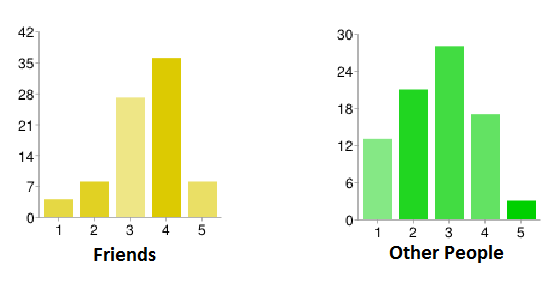
\includegraphics[width=0.8\textwidth]{Images/people.png}
\caption{Graph showing how much people weigh recommendations from their friends and other people}
\label{People}
\end{figure}

The questionnaire started by asking three simple questions about how they weigh specifically peoples opinions when it comes to new media, including their friends, strangers, and themselves.. From the responses it is clear that they weigh their friends recommendation higher than strangers, which mainly got a 4, and strangers lower with a 3. The total spread can be seen in \ref{People} In the final of the three question it was asked if they weigh their own opinion higher than their friends, and the answer was clear, that they do listen to themselves firstmost, rather than to their friends, when it comes to a new piece of media, which can be seen in \ref{Own}.

\begin{figure}[htb]
\centering
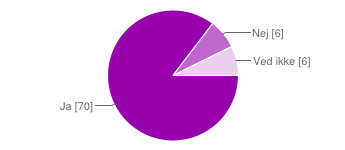
\includegraphics[width=0.8\textwidth]{Images/own.png}
\caption{Graph showing how many people weigh their own opinion higher that any other people}
\label{Own}
\end{figure}

Then the questionnaire proceeded to ask more specific question about different types of media, namely movies, books, music and video games. It asked them how high they weigh a certain factor regarding a type of media, like the director of a movie. Something that was present through all the different types of media, was that the genre of the media had a clear high weight, almost universally, when picking a new piece of media. Genre was also clearly superior compared to every other factor for a genre. Besides genre, there was also other, more niche, factors to take into consideration.
If we look more directly on the different media we can see that:

\textbf{Movies:}

Factors like who directed the movie had a moderately high weight, together with which actors was part of the cast. These two was the most prominent, where the last one was other associated people.

\textbf{Books:}

For books, besides genre, only the author was asked about. The author had a moderate weight for people, but still seems to be quite important for many people.

\textbf{Music:}

When it comes to music, it seems only the specific performer of the song weights highly, while other associated people have a low weight.

\textbf{Video Games:}

Besides the genre, only which studio made the video game had a high weight. Unlike music and movies, actors and voice actors had a very low weights for video games.

People seems to be looking for trending and know details about a piece of media, like the name of a certain actor or actress, a studio, an artist, etc. Most people seems to favor the more apparent factors of a media, like the actors in a movie, rather than the more obscure, like voice actors in a video game. It is also clear that they weigh their own opinion higher, but still hold other peoples opinions to some regard.